\documentclass[a4j]{jarticle}
\usepackage{graphicx}
\usepackage{verbatim}
\usepackage{ascmac}
\usepackage{url}
\usepackage{listings,jlistings}
\usepackage{color}
%\setlength{\marginparwidth}{20mm}%% 傍注欄の横幅の設定

\input{/home/ryousuke/listings_temp.tex}

\title{情報科学プロジェクト実験レポート課題}
\author{S142063 佐藤涼亮}

\begin{document}
\maketitle
\begin{center}
{\LARGE \underline{正規表現}}
\end{center}
\section{課題の内容}
{\large \underline{正規表現による特定の文字列を取り出すプログラムの作成}}
\subsection{要点}
\begin{itemize}
\item C++11で追加された正規表現の指定方法であるstd::ECMAScript構文を使用。
\item 標準入力でhtmlの内容を入力する。
\item 入力されたhtmlの食品アレルギーの原因の文字列を取り出す。
\item 日本語を用いるためワイド文字列を使用する。
\end{itemize}
\section{プログラムの説明}
今回、正規表現による日本語を含めた文章の字句解析を行う。
しかし、日本語のように、漢字(2バイト文字)を含むマルチバイト文字列に対して解析を行うのは困難である。
そこで、Unicodeのようなワイド文字列を用いることで解析を容易に行うことができる。
ワイド文字列は、全ての文字を固定長に変換してしまうものである。
\newpage

htmlの内容を標準入力により一行ずつ読み取る。
読み取った文章をワイド文字列に変換する。
文字列を字句解析し、不要な部分を取り除く。
取り除き方は次のとおりである。\\
\\
\centerline{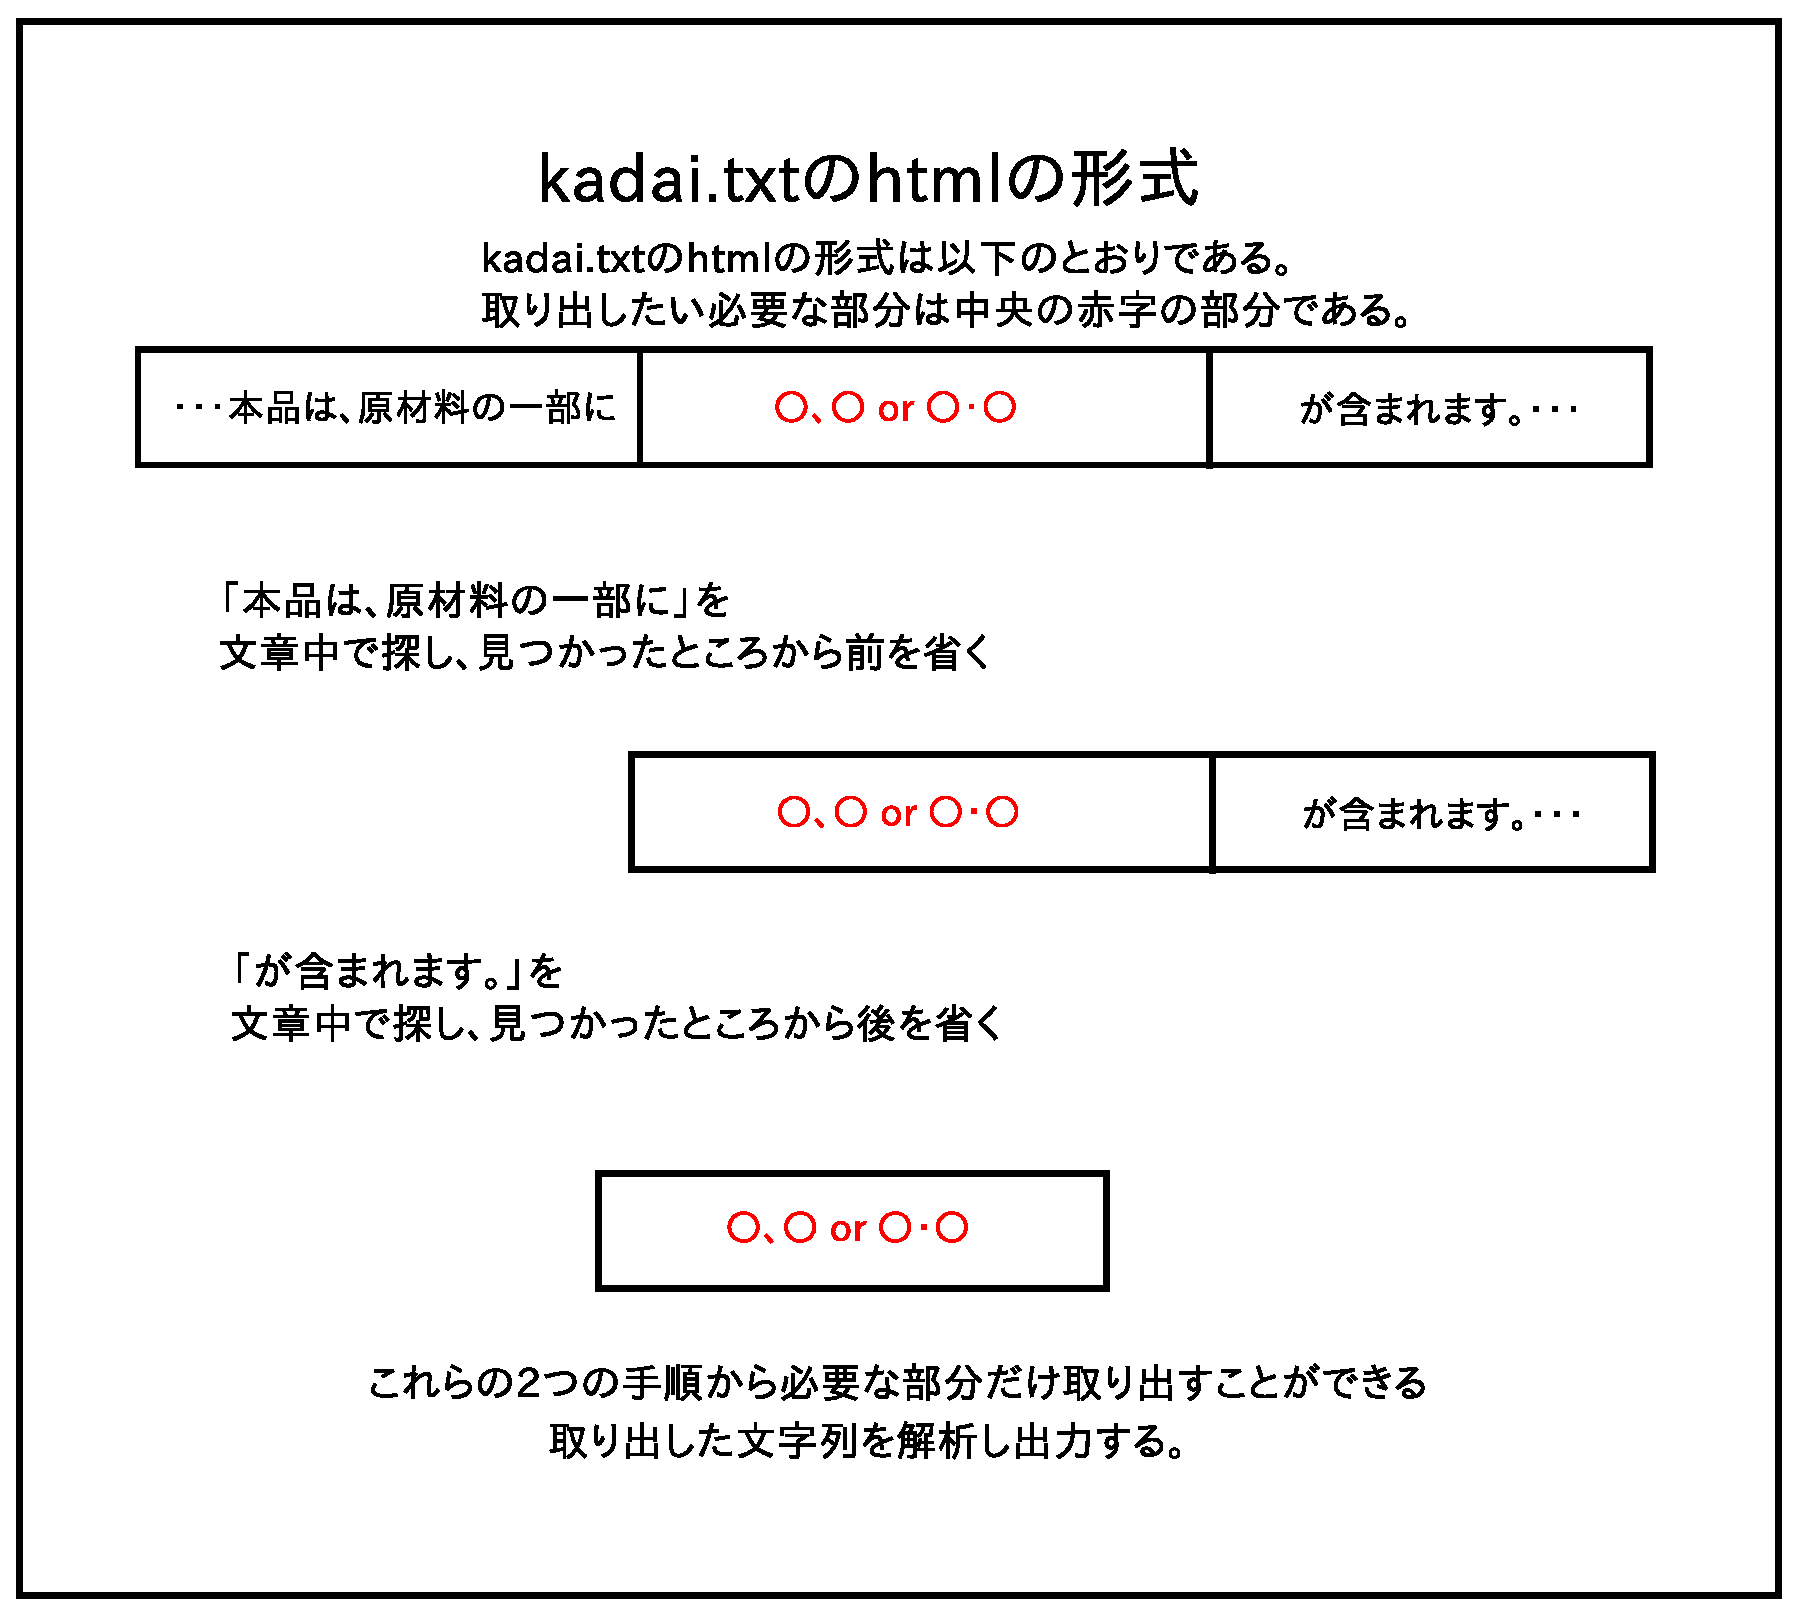
\includegraphics[width=15cm]{dia1.eps}}
\\
取り出した部分の解析には、 \verb|(([^、・]+)[・、]?)| の原材料の解析パターンを使い行う。
原材料の解析パターンでは、
マッチした全体 \verb|(([^、・]+)[・、]?)| が0番目、
原材料のみ \verb|([^、・]+)| が
result\footnote{マッチした情報を格納するクラス}の1番目に格納される。


\subsection{目的}
C++11で追加された正規表現の指定方法であるstd::ECMAScript構文について学ぶ。

\subsection{方法}
htmlに含まれる、食品アレルギーの原因の文字列を、
C++11で追加された正規表現の指定方法であるstd::ECMAScript構文を用いて取り出すプログラムの作成。

\subsection{結果}
実行結果
\begin{screen}
\begin{verbatim}
$ ./report < kadai.txt
えび かに さけ 鶏肉 
乳 
大豆 ゼラチン 
$
\end{verbatim}
\end{screen}
原材料のみの出力に成功した。
\subsection{考察}
原材料のみの出力、およびkadai.txtの実行結果と同じ結果が得られた。

\section{感想}
プログラミング言語の授業で、正規表現を学んだことがあったが、
今回は、std::ECMAScript構文といことで、少し異なった正規表現を学ぶことができた。
今までは、マルチバイト文字のみの文字列を字句解析など解析してきたが、
ワイド文字に変換することで日本語の解析も行えること学んだ。
これらを深く理解することで、インターネットブラウザに標準で備わっている検索機能と同じようなものが作れるのではないかと興味が湧いた。

\newpage
\section{プログラム}
\lstinputlisting[caption=report.cpp,label=report.cpp]{report.cpp}
\section{追記}
別のパターンでプログラムを作成し、同じ結果を得ることができた。
\\
\centerline{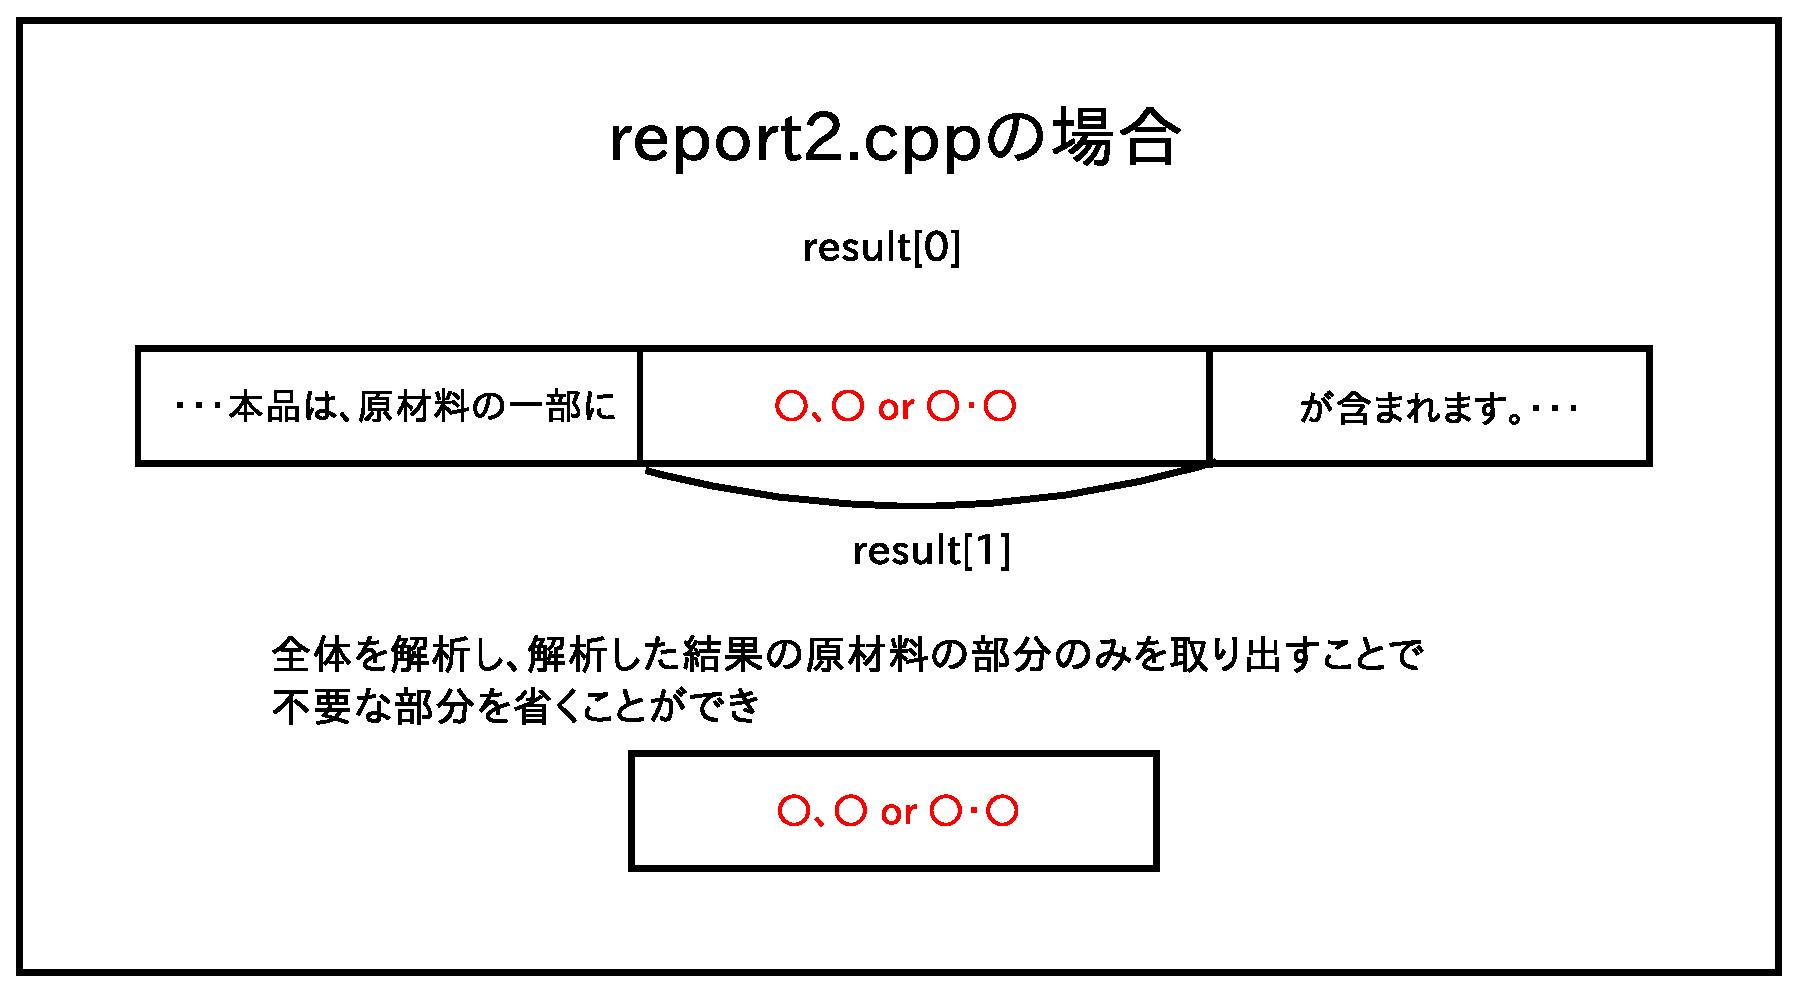
\includegraphics[width=15cm]{dia2.eps}}
\\
\lstinputlisting[caption=report2.cpp,label=report2.cpp]{temp.cpp}

\end{document}
